% =========================================
% CHAPTER 4: System Design and Architecture
% =========================================


\label{chapter:design}

\section{Overview}
\label{sec:design:overview}
This chapter describes the architectural design of the MedEcho system. The solution is 
implemented as a hybrid desktop application combining a responsive frontend interface for 
clinicians with a robust backend responsible for AI processing, data management, and PDF 
report generation.

The architecture follows a modular, scalable, and secure structure to ensure maintainability 
and reliability in real-world hospital deployments.

\section{System Architecture}
\label{sec:design:architecture}
MedEcho uses a \textbf{Client–Server} architecture:

\begin{itemize}
    \item \textbf{Frontend (Client)}: Electron-based interface used by clinicians.
    \item \textbf{Backend (Server)}: Python FastAPI engine responsible for audio processing, 
          LLM structuring, and PDF generation.
    \item \textbf{Data \& Intelligence Layer}: Local Knowledge Layer (LKL), memory storage, 
          and external AI APIs.
\end{itemize}
\subsection*{Architectural Rationale}

The client–server architecture was selected to separate user interaction from AI processing and data management. This separation allows the frontend to remain responsive during heavy AI inference tasks while enabling the backend to scale, optimize, or be replaced independently without affecting the user interface. The layered structure also improves maintainability and supports future integration with hospital information systems.

\subsection{High-Level Architecture Diagram}

The full architecture consists of three layers:

\begin{enumerate}
    \item \textbf{Presentation Layer (Frontend):} Electron + JavaScript + Tailwind CSS.
    \item \textbf{Application Logic Layer (Backend):} Python + FastAPI.
    \item \textbf{Data and Intelligence Layer:} Whisper, GPT-4o, LKL, and memory.json.
\end{enumerate}

\begin{figure}[H]
    \centering
    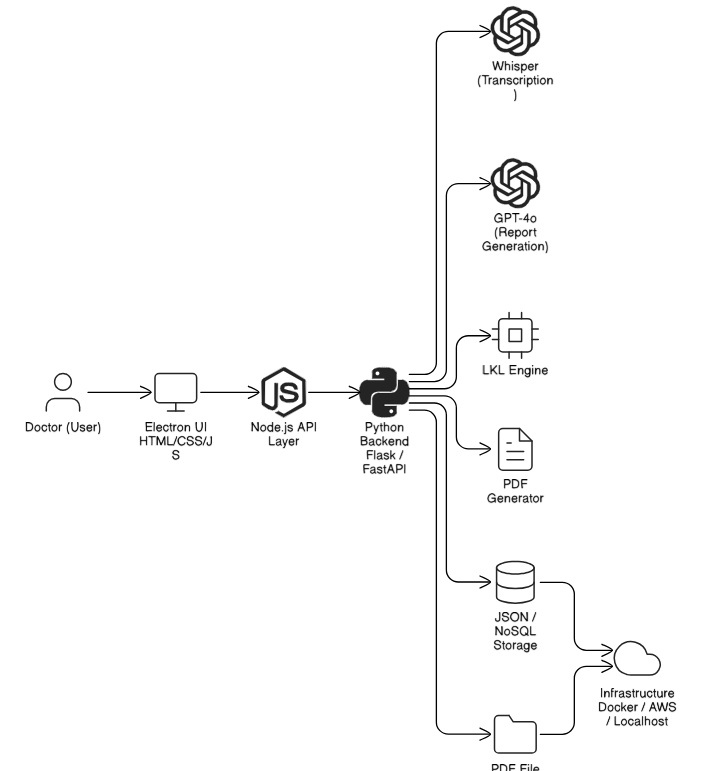
\includegraphics[width=\textwidth]{img/diagram-export-11-30-2025-1_46_10-AM.png}
    \caption{System architecture overview.}
    \label{fig:architecture}
\end{figure}

\section{Component Description}
\label{sec:design:components}
\subsection{Frontend Subsystem}
\label{sec:design:frontend}

\textbf{Technology Stack:} Electron.js, JavaScript, Tailwind CSS.

\subsubsection*{Responsibilities}
\begin{itemize}
    \item \textbf{Dashboard:} Displays patient cases and provides quick navigation.
    \item \textbf{Audio Capture:} Records microphone input, manages start/stop controls, and uploads audio to the backend.
    \item \textbf{Two-Phase Interface:}
    \begin{itemize}
        \item Phase 1 (Intake): Displays AI-generated structured OSCE history.
        \item Phase 2 (Assessment): Allows doctors to review and complete final assessment.
    \end{itemize}
    \item \textbf{Real-Time State Management:} Updates the UI as transcription and LLM processing occur.
\end{itemize}

\subsection{Backend Subsystem}
\label{sec:design:backend}

\textbf{Technology Stack:} Python, FastAPI.

\subsubsection*{Responsibilities}
\begin{itemize}
    \item \textbf{API Endpoints:} Provides routes such as \texttt{/phase1-transcribe}, 
          \texttt{/phase2-final}, \texttt{/generate-pdf}.
    \item \textbf{AI Pipeline Orchestration:} 
          Whisper → Transcript → GPT-4o → Structured JSON.
    \item \textbf{Memory Management:} Saves intake and final assessment cases to \texttt{memory.json}.
    \item \textbf{PDF Engine:} Converts final JSON into a hospital-standard PDF using 
          ReportLab or FPDF.
\end{itemize}

\subsection{AI \& Intelligence Layer}
\label{sec:design:ai}

The AI and Intelligence Layer is responsible for transforming raw clinical speech into structured, clinically valid medical documentation. It combines automatic speech recognition, large language models, and domain-specific grounding to achieve high accuracy, robustness, and contextual consistency.

\subsubsection*{Speech-to-Text (Whisper)}

MedEcho employs OpenAI’s Whisper model for multilingual automatic speech recognition (ASR). Whisper is configured to handle mixed Arabic--English clinical dictation and specialized medical terminology. The model provides low Word Error Rate (WER) even in noisy clinical environments, making it suitable for real-world outpatient and emergency room usage.

\subsubsection*{Large Language Model (GPT-4o)}

GPT-4o acts as the core reasoning and structuring engine of MedEcho. Its main functions include:

\begin{itemize}
    \item \textbf{Entity Extraction:} Identification of OSCE components such as Chief Complaint (CC), History of Present Illness (HPI), Review of Systems (ROS), Past Medical History (PMH), and Medications.
    \item \textbf{Denoising and Filtering:} Removal of irrelevant conversational fillers, repetitions, and non-clinical speech from the transcript.
    \item \textbf{Structured Generation:} Mapping free-text clinical narratives into strict, machine-readable JSON schemas using zero-shot and few-shot prompt engineering.
\end{itemize}

This structured generation enables downstream validation, storage, and PDF report creation while ensuring consistency across different cases.

\subsubsection*{Local Knowledge Layer (LKL)}

The Local Knowledge Layer (LKL) functions as a domain adaptation and grounding component for the LLM. It stores hospital-specific terminology, frequent diagnoses, symptom patterns, and correction rules derived from previously validated cases. During inference, selected LKL entries are injected into the LLM prompt, allowing the system to generate outputs that are aligned with local clinical practice. This approach significantly reduces hallucinations and improves clinical relevance without requiring retraining of the base language model.


\subsubsection*{Local Knowledge Layer (LKL)}

The Local Knowledge Layer (LKL) acts as a domain adaptation and grounding mechanism for the LLM. It stores hospital-specific terminology, frequent diagnoses, symptom patterns, and correction rules derived from previously processed cases. During report generation, selected LKL entries are injected into the LLM prompt, enabling contextual grounding, reducing hallucinations, and improving consistency with local clinical practice without requiring retraining of the base language model.

\begin{itemize}
    \item Continuously accumulates hospital-specific clinical patterns from processed cases.
    \item Provides domain grounding to the LLM during inference to reduce hallucinations.
    \item Adapts report generation to local terminology and documentation style.
    \item Enhances longitudinal consistency across multiple patient encounters.
\end{itemize}

\section{Data Flow Design}
\label{sec:design:dataflow}

The data flow of MedEcho occurs in five main stages:

\subsection*{1. Input}
Doctor records audio (Phase 1 intake or Phase 2 final assessment) through the Electron UI.

\subsection*{2. Transmission}
Audio is uploaded to the FastAPI backend using an HTTP POST request.

\subsection*{3. Processing}
\begin{enumerate}
    \item Whisper transcribes the audio.
    \item Backend sends transcript + LKL context to GPT-4o.
    \item GPT-4o returns structured JSON (intake or final report).
\end{enumerate}

\subsection*{4. Review}
Structured JSON is returned to the Electron UI for clinician verification.

\subsection*{5. Finalization}
When approved:

\begin{itemize}
    \item JSON is saved to \texttt{memory.json}.
    \item LKL updates with new findings.
    \item A final PDF is generated and shown to the user.
\end{itemize}

\begin{figure}[H]
    \centering
   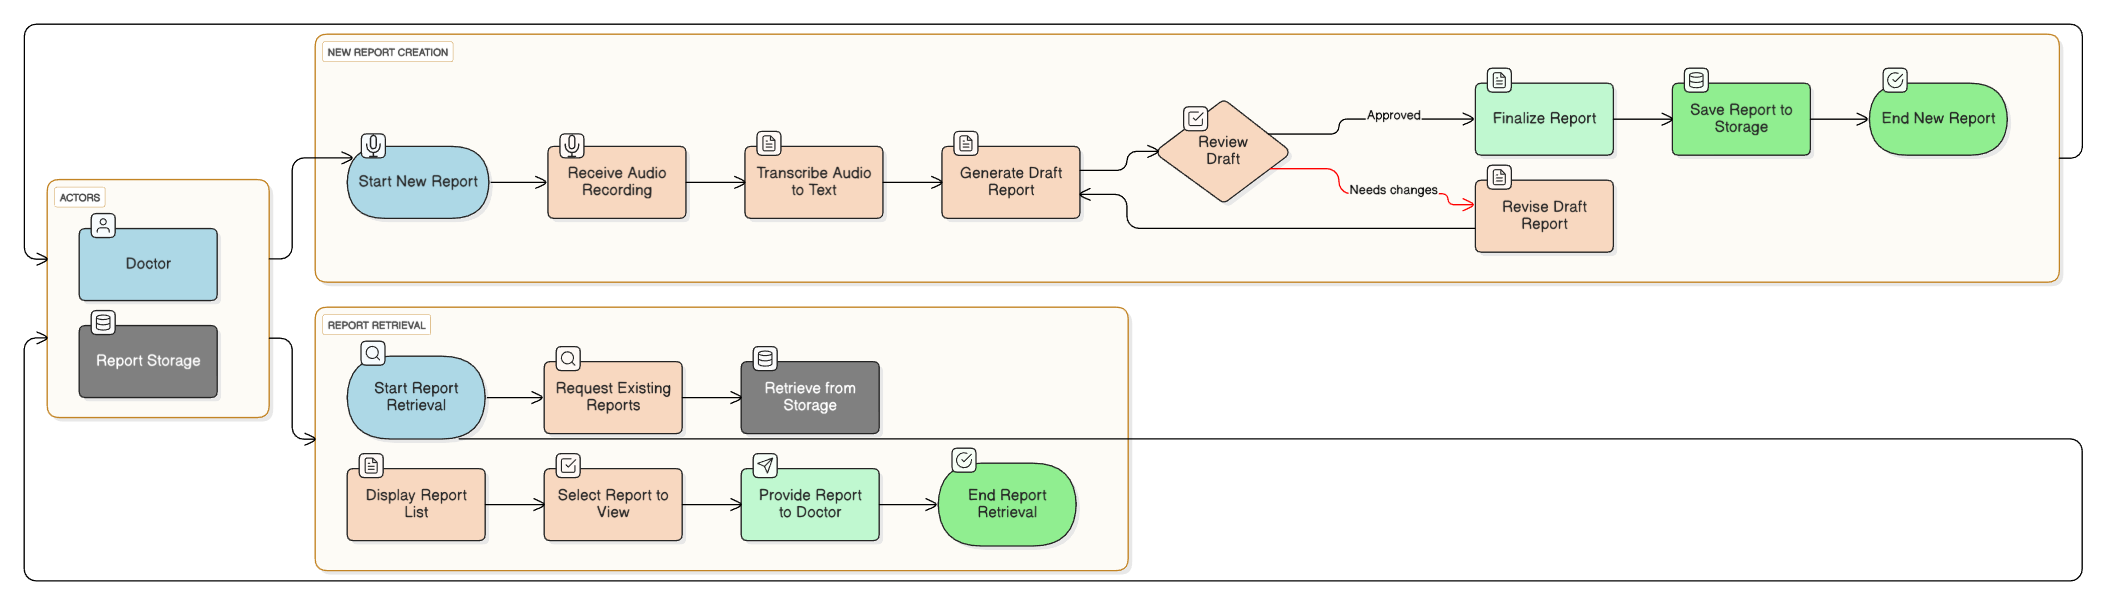
\includegraphics[width=\textwidth]{img/dfd 0.png}
    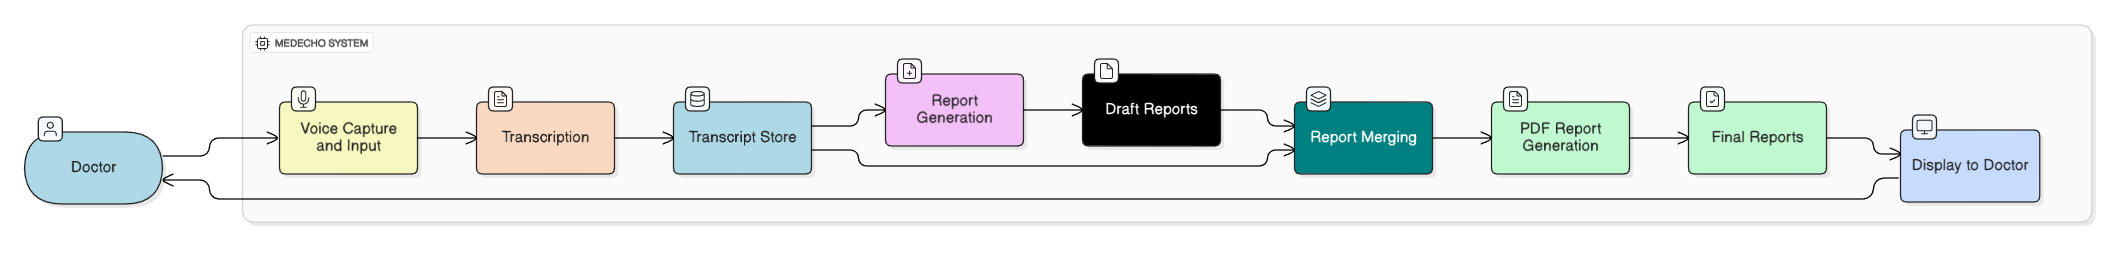
\includegraphics[width=\textwidth]{img/dfd 1.png}
    \caption{Data processing workflow in MedEcho.}
    \label{fig:dataflow}
\end{figure}
